\documentclass[11pt]{article}
\usepackage{royden-report}
\usepackage[T1]{fontenc}
\usepackage{lmodern,microtype,array}
\newcommand{\D}{\lvert D_\tau\rvert}
\newcommand{\HH}{\mathcal H}
\newcommand{\TT}{\mathbb T_L}
\newcommand{\norm}[1]{\lVert #1\rVert}
\newcommand{\abs}[1]{\lvert #1\rvert}
\newcommand{\dd}{\,\mathrm d}
\newcommand{\F}{\mathcal F}
\title{Dysthe Evolution: Numerical Evidence and Existence}
\author{}
\date{23 October 2026}
\hypersetup{pdftitle={Dysthe Evolution: Numerical Evidence and Existence},
pdfsubject={Review of two water-wave papers and a numerical/PINN existence research plan}}
\begin{document}
\maketitle
\begin{abstract}
The recommended first project is a study of continued smooth evolution
for the approved spatial free-surface water-wave Dysthe equation, using
a qualified Fourier solver and a separately evaluated physics-informed
neural network (PINN). The immediate output should be a reproducible map
of resolved propagation intervals, derivative growth, and approximation
error. An existence theorem requires additional control of stability
and unresolved modes. We review Dysthe (1979) and Schober--Islas (2026,
supplied version 1), identify two apparent linear-dispersion
inconsistencies in the latter, and show why a real delayed mean flow is
not automatically equivalent to its complex damping model.
No new evolution campaign, trained PINN, or computer-assisted existence
certificate is claimed here.
\end{abstract}

\section{The research target}
The question is whether prescribed smooth envelopes remain smooth as
time or propagation distance increases. It is not primarily a search
for solitary waves. Three tasks must be distinguished:
\begin{enumerate}
\item Construct a numerical trajectory and a PINN approximation for the
same equation, initial data, domain, and interval.
\item Assess continued regularity by checking derivative norms, spectra,
and the full equation residual under independent refinement.
\item Prove existence through a matching local theory and continuation
estimate, or a rigorous a posteriori validation of a trajectory.
\end{enumerate}
A successful first project can complete the first two tasks and prepare
the third. A smooth plot, agreement between two methods, or a small
training loss does not by itself complete the third.

\paragraph{Recommendation.}
Begin with \texttt{water-wave-dysthe-spatial-v1}, which already has a
working reference solver. Use short propagation windows and a
Fourier-in-profile PINN. Evaluate both methods using the full residual,
including discarded frequencies. Target a rigorous certificate on one
short periodic interval before attempting an all-distance claim.
Keep the newer paper's temporal damping and relaxation constructions
separately identified; do not insert them into the approved baseline by
changing a coefficient.

The useful research result is: for a specified family of initial
water-wave envelopes, how far are the approximations trustworthy,
which derivatives grow first, what limits that interval, and can a
rigorous bound certify at least one trajectory?

\section{What the supplied papers establish}
\subsection{Dysthe (1979): a model and a stability calculation}
Dysthe derives corrections beyond cubic nonlinear Schr\"odinger (NLS)
theory from inviscid, irrotational, deep-water free-surface flow
\cite{dysthe}. His \(A\) is a velocity-potential envelope. The full
system, printed equations (2.19)--(2.21) with the mean-flow Laplace
equation, evolves in time and includes two horizontal coordinates.
It is not the project's spatial free-surface equation.

Slow modulation drives an induced mean potential. Its horizontal
current changes the local carrier frequency and modifies sideband
instability. Section 3 linearizes about a uniform wavetrain.
For example, equation (3.10), printed p.~111, gives
\[
 \gamma_M=\tfrac12(1-2A_0)A_0^2,
\]
where \(A_0\) is nondimensional carrier steepness. Figures 1--3 compare
approximate instability predictions with previous calculations and
measurements. These are not convergence tests of nonlinear trajectories.

The simplified equations (4.1)--(4.3), printed p.~113, retain the
mechanism responsible for the stated leading stability correction.
They should not replace the full evolution model in a regularity study
without a separate justification. The paper supplies neither a
well-posedness theorem nor a rigorous approximation-error theorem
relative to the Euler equations.

\begin{remark}
Modulational instability means that certain small disturbances grow.
It does not imply blow-up or nonexistence. Conversely, a smooth
envelope solution need not stay within the weak-steepness, narrowband
regime in which the water-wave approximation is physically credible.
\end{remark}

\subsection{Schober--Islas (2026): three distinct constructions}
The supplied preprint \cite{schober} must be read as three constructions.
\begin{enumerate}
\item Its introductory equation (1.1) is a phenomenological temporal
model with a complex coefficient in the nonlocal interaction:
\begin{equation}
 i u_t+u_{xx}+2|u|^2u+
 \epsilon\left[2u(1+i\beta)\HH\partial_x(|u|^2)
 -8i|u|^2u_x+\tfrac i2u_{xxx}\right]=0.
 \label{eq:beta}
\end{equation}
The paper identifies \(\beta=0\) with a Hamiltonian Dysthe formulation.
Its variable is not automatically the 1979 potential envelope or the
approved spatial free-surface envelope.
\item Sections 2--6 use the Dias--Dyachenko--Zakharov (DDZ)
potential-flow reduction with weak viscosity
\(\bar\nu=\epsilon^2\nu\). The reported fifth-order calculation produces
derivative-dependent nonlocal terms but no explicit viscosity
multiplier on the leading mean-flow operator. The sixth-order
calculation isolates one carrier--mean contribution; it does not
derive the complete sixth-order equation or the final net coefficient.
\item Section 7 introduces an independent relaxation closure for the
mean flow. It is not derived from the DDZ hierarchy. Its adjustment
time is prescribed, with physical origin and calibration unresolved.
\end{enumerate}
The preprint does not derive a constant positive \(\beta\) from first
principles and does not establish existence or continued smoothness.
Its fifth-order cancellation is a conclusion of its formal expansion;
we have not independently reproduced the full harmonic calculation.
The paper itself distinguishes asymptotic order and operator structure
from a term-by-term identification with its introductory equation.

\subsection{Two apparent inconsistencies in the supplied version}
The following findings were checked against the rendered PDF. They
motivate a source/author audit, not an unannounced repair of the model.

\paragraph{Cubic dispersion.}
Equation (4.14), p.~9, prints
\[
 -\epsilon^2\frac{8ik^3}{\omega^2}A_{XXX}.
\]
For the stated dimensional \(X=\epsilon x\), \(T=\epsilon t\),
\(\omega^2=gk\), and carrier \(e^{i(\omega t-kx)}\), the coefficient
is dimensionally inconsistent. Independently, put
\(A=e^{i(KX-\Omega T)}\) and remove viscosity and nonlinearity.
Exact deep-water dispersion requires
\begin{align}
 \Omega
 &=\frac{\omega-\sqrt{g(k-\epsilon K)}}{\epsilon} \notag\\
 &=\frac{\omega K}{2k}
 +\epsilon\frac{\omega K^2}{8k^2}
 +\epsilon^2\frac{\omega K^3}{16k^3}
 +\epsilon^3\frac{5\omega K^4}{128k^4}
 +O(\epsilon^4).
 \label{eq:dispersion}
\end{align}
In the paper's normalization
\(2i\omega(A_T+\omega A_X/(2k))+\cdots=0\),
the cubic coefficient consistent with this expansion is
\(-i\omega^2/(8k^3)\), not \(-8ik^3/\omega^2\).
Even at \(k=\omega=1\), their magnitudes differ by a factor of 64.

\paragraph{Missing quartic dispersion.}
Equations (5.6), (5.7), and (5.11), p.~12, claim a complete fifth-order
condition, but their inviscid linearization contains no \(A_{XXXX}\).
In the same variables, \eqref{eq:dispersion} requires
\(-5\epsilon^3\omega^2 A_{XXXX}/(64k^4)\).
No exact-dispersion operator or documented change of envelope variable
explaining this absence was identified.

These are apparent inconsistencies in the supplied version, not a
rederivation of its nonlinear hierarchy. Check possible corrections
and the complete linear DDZ dispersion before implementing the
higher-order equation. Correcting two terms would not validate
all remaining coefficients.

\section{Real mean-flow delay is not automatically nonlinear damping}
Adopt \(\widehat{\HH f}(k)=-i\operatorname{sgn}(k)\widehat f(k)\),
so \(\HH\partial_x=|D_x|\).
Write \(\theta>0\) for the relaxation time called \(\tau\) in the
new paper, avoiding confusion with the project's retarded time.
Its equations (7.1)--(7.2) are
\begin{equation}
 M_0=-\frac{2k^2}{\omega}\HH\partial_X|A|^2,\qquad
 \theta M_T+M=M_0.
 \label{eq:relax}
\end{equation}
For real forcing and real initial \(M_{\rm in}\),
\begin{equation}
 M(T)=e^{-T/\theta}M_{\rm in}
 +\theta^{-1}\int_0^T e^{-(T-s)/\theta}M_0(s)\dd s
 \label{eq:convolution}
\end{equation}
is real. An initial-value simulation must specify \(M_{\rm in}\);
a steady harmonic transfer function omits this transient.

For time dependence \(e^{-i\Omega T}\),
\[
 G(\Omega)=\frac1{1-i\Omega\theta},\qquad
 G(-\Omega)=\overline{G(\Omega)}.
\]
Its low-frequency approximation is \(1+i\Omega\theta\).
In physical time this corresponds to
\[
 M=M_0-\theta\,\partial_T M_0+O(\theta^2),
\]
under appropriate temporal regularity and with the initial layer
accounted for. It remains real. Replacing the entire real signal by
\((1+i\beta)M_0\), for a constant positive \(\beta\), does not preserve
the required conjugate symmetry. A selected complex Fourier amplitude
can have such a phase lag; that does not establish equality of the
full nonlinear models.

\begin{figure}[htbp]
\centering
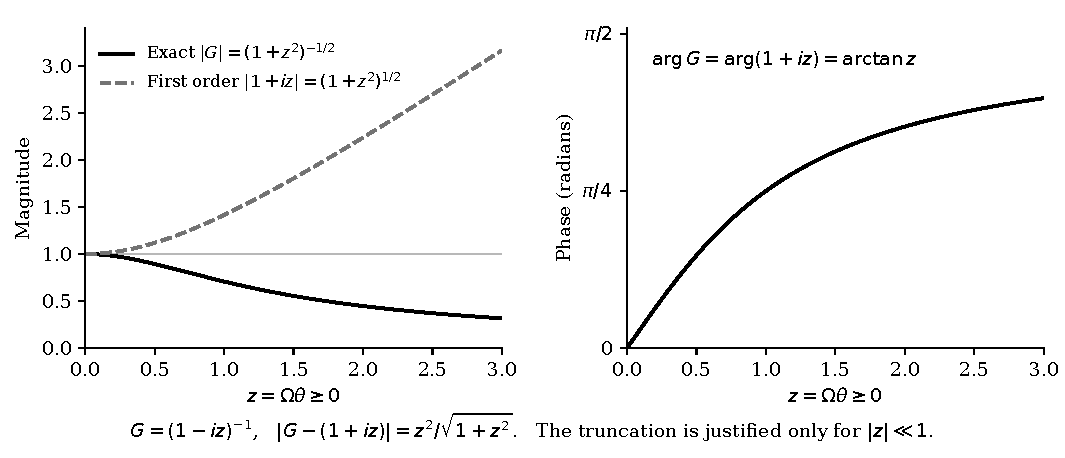
\includegraphics[width=.94\linewidth]{figures/phase_lag_response.pdf}
\caption{Analytic relaxation response for \(z=\Omega\theta\).
The exact and first-order transfer functions have the same phase,
but different magnitudes. These are analytic curves, not simulated
wave trajectories.}
\end{figure}
Indeed \(G=(1+iz)/(1+z^2)\), so
\[
 |G-(1+iz)|=\frac{z^2}{\sqrt{1+z^2}}.
\]
The assumption \(\Omega\theta=O(\epsilon)\) places the correction
one order beyond Dysthe; it is an imposed asymptotic ordering,
not a measured adjustment time.

\begin{proposition}[Mass balance for the complex-coefficient model]
Let \(u\) be a sufficiently smooth \(L\)-periodic solution of
\eqref{eq:beta}, with real \(\epsilon,\beta\). Set
\(\rho=|u|^2\), \(Q(t)=\int_0^L\rho\dd x\).
Then
\begin{equation}
 Q'(t)=-4\epsilon\beta\int_0^L\rho\,|D_x|\rho\dd x
 =-4\epsilon\beta\norm{|D_x|^{1/2}\rho}_{L^2}^2.
 \label{eq:mass-beta}
\end{equation}
\end{proposition}
\begin{proof}
Differentiate \(Q\) to obtain \(2\operatorname{Re}\int\bar u u_t\).
The dispersive terms and the purely imaginary multiplication terms
have zero real integral. The derivative nonlinearity gives a
multiple of \(\int\rho\rho_x=0\).
The remaining contribution to \(u_t\) is
\(-2\epsilon\beta u|D_x|\rho\). Parseval's identity gives the
last equality because the multiplier \(|k|\) is nonnegative.
\end{proof}
By contrast, a real \(M\) multiplying \(u\) with a real coefficient
in the \(iu_t\) equation contributes zero to \(Q'\).
Replacing the real mean term of the \(\beta=0\) equation by such
a relaxing \(M\) therefore preserves envelope mass. Additional
viscous terms can change this conclusion; the comparison isolates
the mean-flow mechanism.
Delay may affect phase and other energy exchanges, but it does not
produce \eqref{eq:mass-beta} through this substitution.

Even \eqref{eq:mass-beta} does not prove global smoothness. It bounds
mass and a time-integrated half derivative of \emph{intensity},
not all derivatives of the envelope. For example, \(|a e^{inx}|^2\)
is constant although its envelope derivatives grow with \(n\).
This is a mathematical demonstration of missing control; arbitrarily
large \(n\) violates narrowband physics.

\section{Freeze the equation and the meaning of smoothness}
The approved periodic spatial initial-value problem is
\begin{align}
 u_\xi=F(u)&=-iu_{\tau\tau}-i|u|^2u \notag\\
 &\quad-\epsilon\left(8|u|^2u_\tau+
 2u^2\overline{u_\tau}+2iu\D(|u|^2)\right),\label{eq:baseline}\\
 u(0,\tau)&=u_0(\tau),\qquad \tau\in\TT=\RR/(L\ZZ).
 \label{eq:initial}
\end{align}
Here \(\xi\) is propagation distance, \(\tau\) retarded time,
and \(u\) the scaled free-surface envelope. In the contract's
carrier units, \(\tau=\epsilon(2x-t)\), \(\xi=\epsilon^2x\),
and \(B=\epsilon u\).
For \(k_m=2\pi m/L\), \(\D\) has multiplier \(|k_m|\)
and zero mean mode. The coefficient 2 of
\(u^2\overline{u_\tau}\) must not be replaced by the
potential-envelope value 0.
This is the local contract's Fedele--Dutykh spatial convention
\cite{fedele}.

For \(u=\sum_m a_m e^{ik_m\tau}\), set
\[
 \norm{u}_{H^s(\TT)}^2=L\sum_m(1+k_m^2)^s|a_m|^2.
\]
The intended finite-interval claim must specify a class, such as
\(C([0,\Xi];H^s(\TT))\). Well-posedness additionally requires
uniqueness and continuous dependence in the stated spaces.
The diagnostic choice \(s=3\) below is not claimed to be a
known optimal existence threshold.

\section{A numerical study of continued smoothness}
\label{sec:numerical-campaign}

The first computational question should be precise: for specified smooth
initial packets, how far can solutions of \eqref{eq:baseline} be followed with
resolved derivatives and reproducible error estimates?  A successful finite
interval supplies evidence of continued smooth behavior on that interval.
Extending the interval does not by itself establish global existence.

\subsection{What can already be reused}

The local \texttt{dysthe-core} reference evolves the approved spatial equation
on a periodic profile interval of length $L$, with Fourier differentiation,
retained modes $|m|<N/4$, and integrating-factor fourth-order Runge--Kutta
steps in $\xi$.  Its independent controls include the linear symbol, a nonzero
wavenumber plane wave, the exact NLS traveling profile, and a direct Fourier
convolution of the nonlinear terms including mean flow.  The local
\texttt{dysthe-experiments} code already supplies matched controls,
phase/translation alignment, full periodic residual checks, and separate
grid, step, and domain comparisons.

Stored results for $\epsilon=.025$, $L=160$, $N=4096$,
$h=\Delta\xi=.00125$, and $0\leq\xi\leq4$ give the following maximum raw
complex relative $L^2$ discrepancies.  Each input was compared separately
with $2N$, with $h/2$, and with $2L,2N$ at fixed profile spacing.
\begin{center}
\small
\begin{tabular}{lrrr}
\toprule
Initial field & Grid & Step & Domain\\
\midrule
Solitary profile & $4.17\times10^{-15}$ & $3.07\times10^{-9}$ & $1.54\times10^{-6}$\\
Localized $2\%$ perturbation & $3.09\times10^{-15}$ & $4.08\times10^{-9}$ & $2.26\times10^{-6}$\\
Complex Gaussian & $9.28\times10^{-16}$ & $4.05\times10^{-11}$ & $2.18\times10^{-5}$\\
\bottomrule
\end{tabular}
\end{center}
These are existing two-level agreement checks, not rigorous error bounds or
observed convergence orders.  The stored qualification files were inspected
for this review; these trajectories were not rerun.  Fresh unit tests passed
21 of 21 core checks and 43 of 47 experiment checks; four HTTP tests could not
open a socket in the execution sandbox.  Passing tests neither qualifies a
new packet nor proves a PDE theorem.  The reference additions are local
uncommitted work; a reproducible campaign must record their source hashes.

\subsection{A bounded campaign with explicit stopping rules}

Use $\epsilon\in\{0,.025,.05\}$, treating zero as the mathematical NLS
control.  Start with the existing smooth Gaussian and qualified traveling
profiles, then add signed amplitude and phase perturbations outside the
profile-construction symmetry.  Keep all parameters, initial Fourier
coefficients, and initial-condition identifiers fixed within a refinement
comparison.  The first task is a few documented cases, not a large training
dataset.

Start at $(N,L,h)=(4096,160,.00125)$.  Compare $N,2N,4N$ at fixed $L$ with a
separately qualified step; compare $h,h/2,h/4$ at fixed fine grid; enlarge to
$2L$ and, when necessary, $4L$ at fixed profile spacing.  Reconstruct localized
initial data on each domain rather than repeating its periodic copies.
Recomputed solitary profiles must retain and report their initial-domain
discrepancy.  The nonlocal mean flow can change with $L$ even when edge
amplitudes are tiny.

Use successive horizons
\[
  \Xi\in\{1,2,4,8,16,32\},
\]
advancing only after the preceding horizon passes its checks.  Compare all
saved stations and inspect denser output near rapid growth.  Retain raw
complex errors as well as errors after fitting only translation and constant
phase; never fit away amplitude changes.  Perturbations should also be
compared with their matched propagated control.  A failed gate calls for
refinement or a shorter qualified interval; it is not evidence of blow-up
or nonexistence.

For $k_m=2\pi m/L$ and Fourier coefficients normalized by $1/L$, record
\begin{equation}\label{eq:monitor-sobolev}
 \norm{u}_{H^s(\TT)}^2
 =L\sum_m(1+k_m^2)^s|\widehat u_m|^2,
 \qquad s=1,2,3.
\end{equation}
Also record $\norm{u}_{\infty}$, $\norm{u_\tau}_{\infty}$, and spectral
slopes above the resolved signal floor.  Monitor the fraction of each
$H^s$ sum in the upper fifth of the retained band.  A small unweighted
spectral tail can conceal a large derivative error.  Check boundary and
exterior contributions in derivative norms, not action alone.  Apparent
norm growth is interpretable only while these weighted tails, slopes, and
refinement comparisons remain resolved.

Provisional gates are maximum raw relative $L^2$ discrepancy $10^{-4}$,
$H^1$ discrepancy $10^{-3}$, and $H^2,H^3$ discrepancies $10^{-2}$, with
upper-band weighted fractions below $10^{-6}$.  Use the finer field for
normalization and absolute scales when the reference norm is near zero.
For a weak perturbation, additionally require the signed response
discrepancy below $2\%$ of the measured response above its numerical floor.
These are proposed acceptance tolerances, not established error bounds;
tighten them when the scientific effect is smaller.  Step halving must show
the expected order before roundoff, rather than just two close answers.
The existing $\epsilon\norm{u}_\infty$ and bandwidth screens remain
separate physical-model checks; their thresholds are not universal validity
theorems.

Evaluate the unprojected RHS on an enlarged Fourier grid, retaining discarded
nonlinear modes.  For a continuous reconstruction $v$ of a numerical
trajectory, the useful defect is $r=v_\xi-F(v)$, including error from the
reconstruction in $\xi$.  The existing snapshot RHS diagnostic alone does
not provide that time-dependent defect or its integral.  Mass drift is an
additional diagnostic; it cannot replace derivative resolution or residual
control.

\section{A Fourier-in-profile physics-informed network}
\label{sec:spectral-pinn}

\subsection{Represent the periodic field and retain the full residual}

The recommended first PINN is a neural approximation of the Fourier
coefficients as functions of propagation distance:
\begin{equation}\label{eq:spectral-pinn}
 v_\vartheta(\xi,\tau)
 =\sum_{m=-K}^{K}a_m(\xi;\vartheta)e^{ik_m\tau},
 \qquad a_m\in\CC.
\end{equation}
A smooth network takes $\xi$ and returns the real and imaginary parts of
all coefficients.  Periodicity is exact.  Because the envelope is complex,
\emph{do not impose} $a_{-m}=\overline{a_m}$ or conjugate-reflection symmetry.
Choose $K$ from convergence of the reference fields in $H^3$, and repeat
with a larger $K$; action capture alone is insufficient.

Automatic differentiation supplies $a_m'$, while the profile derivatives
use $ik_m$ and $-k_m^2$.  At each sampled $\xi$, form
$\rho=|v_\vartheta|^2$, compute $\D\rho$ with multiplier $|k_m|$ and zero
mean mode, and evaluate every term of \eqref{eq:baseline}.  Define
\begin{equation}\label{eq:pinn-residual}
 r_\vartheta=\partial_\xi v_\vartheta-F(v_\vartheta).
\end{equation}
The cubic terms, including $v_\vartheta\D(|v_\vartheta|^2)$, can contain modes
through $3K$.  The residual must retain these modes even though the trial
field stops at $K$.  A uniform quadrature grid with $Q>6K$ points resolves
this full residual and its squared $L^2$ norm for the trigonometric trial
field.  Penalizing only $|m|\leq K$ could conceal a large discarded RHS and
merely solve a truncated coefficient system.  Independently validate with
larger $Q$, larger $K$, and new propagation stations.

\subsection{Hard initial values and short propagation windows}

On $[\xi_j,\xi_{j+1}]$, write
\[
 a_m(\xi;\vartheta)
 =a_m^{(j)}+(\xi-\xi_j)b_m(\xi;\vartheta).
\]
This enforces the supplied initial coefficients exactly.  On the first
window, report the projection error of the prescribed initial field onto
$|m|\leq K$; a hard condition does not remove this error.  On later windows,
set $a_m^{(j)}$ to the previous learned terminal value.  Errors therefore
accumulate honestly.  Replacing every window's initial value with a
reference snapshot defines a different, data-assisted experiment and must
be reported separately.

Begin with short windows inside $\Xi=1$, double precision, a smooth modest
network, and at least three recorded initialization seeds.  A practical
training sequence is Adam followed by a bounded L-BFGS refinement.  Declare
the architecture, coefficient scaling, optimization budget, window length,
and stopping rules before comparison.  A basic loss is
\[
 \mathcal L_{\rm PDE}
 =\frac{1}{(\xi_{j+1}-\xi_j)L}
   \int_{\xi_j}^{\xi_{j+1}}\int_{\TT}|r_\vartheta|^2\dd\tau\dd\xi.
\]
An explicitly stated Fourier-weighted residual may improve derivative
control, but changes the training objective and must be tested.  Conservation
is a diagnostic rather than a substitute for the PDE loss.  Do not supply
interior reference snapshots to a purported physics-only run; if such data
are used, report that variant alongside it.

\subsection{What would count as a meaningful result}

First require the NLS and plane-wave controls, then the nonconstant mean-flow
case, then the packet campaign.  At held-out stations compare the network
with the refined reference in raw complex $L^2$, $H^1,H^2,H^3$, peak and
profile slope, phase where amplitude is meaningful, and full residual.
Compare matched perturbation responses before interpreting their growth.
Training failure, a small collocation loss, or disagreement between two
networks cannot decide existence.  A residual becomes an error certificate
only when combined with justified stability estimates or validated inverse
bounds of the kind discussed elsewhere in this report.

The active learning repository has no implemented water-wave PINN.  This
review adds no new trajectory or trained network.  Its proposed first
deliverable is one reproducible short-window comparison, followed by horizon
extension only after qualification.  Record total training and evaluation
time, peak memory, all restarts and seeds, and any reference-generation cost;
compare with the numerical solver at matched accuracy.  A PINN has no
presumed speed advantage for this one-coordinate problem.  Its potential
value must come from a demonstrated use---for example, a differentiable
family of accurate approximations---rather than the name of the method.

\section{What would establish continued smooth existence?}
\label{sec:existence}

The question is whether prescribed smooth initial data generate a solution
of \eqref{eq:baseline} that continues to exist with controlled derivatives
as the propagation distance increases. Three claims must be separated:
existence on a specified finite interval; continuation for every finite
distance; and smoothness of all orders. A computation over a finite interval
can support the first claim empirically. Neither a bounded maximum amplitude
nor a bounded $L^2$ norm controls all derivatives.

\subsection{The available theory must match the equation}

Mosincat, Pilod and Saut prove local well-posedness in
$H^s(\mathbb R^2)$, $s>0$, and global well-posedness and scattering for
sufficiently small $L^2(\mathbb R^2)$ data for their \emph{temporal}, nonlocal
Dysthe equation; see their equation~(1.12) and Theorems~1.1--1.2
\cite{mps}. Their one-dimensional whole-line discussion concerns temporal
Dysthe with third-order dispersion and $H^s(\mathbb R)$, $s\geq1/4$.
These statements do not directly cover our second-order spatial equation
on a periodic profile domain. Nonzero constant backgrounds are also outside
the finite-$L^2(\mathbb R^2)$ hypothesis.

For one-dimensional periodic temporal Dysthe, Heller and Shao obtain
estimates and low-regularity ill-posedness results, but explicitly do not
prove local well-posedness of the full equation \cite[\S1.5]{heller}.
Belloni and Giuliani's recent global result for a local periodic
NLS--Dysthe family likewise does not settle our problem: their discussion
explicitly excludes the water-wave mean-flow term $u|D|(|u|^2)$
\cite[pp.~5--6]{belloni}. Thus we have not identified a theorem whose stated
hypotheses match \eqref{eq:baseline}. This is a limitation of the present
review, not a claim that all Dysthe existence questions are open.

\subsection{A rigorous finite-dimensional statement, and its limit}

Let $\TT$ be the periodic profile circle of length $L>0$, and let $P_K$
denote the orthogonal Fourier projection onto modes $|n|\leq K$.
Write $F(u)$ for the full right-hand side of \eqref{eq:baseline}.
The following statement concerns exact Galerkin evolution, with exact
nonlinear products and the stated Fourier mean-flow operator.

\begin{proposition}[Global existence at each fixed Fourier cutoff]
\label{prop:galerkin-global}
Let $K$ be a nonnegative integer, let $\epsilon\in\mathbb R$, and let
$u_K(0)$ belong to the range of $P_K$. The finite system
\[
  \partial_\xi u_K=P_KF(u_K)
\]
has a unique solution for every $\xi\in\mathbb R$, and
$\norm{u_K(\xi)}_{L^2(\TT)}=\norm{u_K(0)}_{L^2(\TT)}$.
\end{proposition}
\begin{proof}
Its Fourier coefficients solve a polynomial ordinary differential
equation in finitely many real variables, hence have a unique local
solution. Put $\rho=|u_K|^2$. Self-adjointness of $P_K$ and $P_Ku_K=u_K$
allow its removal from the mass derivative. The linear dispersive term
vanishes after integration by parts. The local cubic term and the mean-flow
term have zero real contribution because $\rho$ and $|D_\tau|\rho$ are real.
The remaining two derivative terms give
\[
 \frac{\dd}{\dd\xi}\norm{u_K}_{L^2}^2
 =2\operatorname{Re}\int_{\TT}\overline{u_K}F(u_K)\,\dd\tau
 =-10\epsilon\int_{\TT}\rho\,\partial_\tau\rho\,\dd\tau=0.
\]
Parseval's identity therefore bounds the coefficient vector throughout
its maximal interval. In finite dimension it remains in a compact ball,
where the polynomial vector field and its derivative are bounded.
The ordinary differential equation continuation theorem excludes a finite
endpoint in either direction.
\end{proof}

This proposition does not prove existence for the partial differential
equation, or stability of a chosen time-stepping method. For $s>0$ it gives
only
\[
 \norm{u_K(\xi)}_{H^s(\TT)}
 \leq\left(1+\left(\frac{2\pi K}{L}\right)^2\right)^{s/2}
       \norm{u_K(0)}_{L^2(\TT)},
\]
whose constant grows with $K$. Global finite systems can therefore fail
to provide the uniform regularity needed in the limit $K\to\infty$.
An aliased implementation need not equal this Galerkin system, and an
RK4 update does not inherit its exact mass conservation or global bound.

\subsection{The analytic continuation route}

A PDE proof must first establish local existence, uniqueness and
continuous dependence in a specified function space for the exact
equation and boundary conditions. Directly applying a finite-dimensional
ODE argument is insufficient: the nonlinear terms contain derivatives,
including the first-order nonlocal operator $|D_\tau|$, so a naive
same-$H^s$ nonlinear estimate loses derivatives. Suitable cancellations,
modified energy estimates, or dispersive estimates must recover this loss.

If a local theory supplies a lifespan bounded below in terms of the
$H^s$ norm, its restart argument gives a continuation criterion: a finite
maximal distance can occur only if that controlling norm becomes
unbounded. Establishing the needed norm bound uniformly on every finite
interval would then give global existence in that regularity class.
Passing from Galerkin approximations also requires sufficient compactness,
convergence of the derivative nonlinearities, and uniqueness of the limit.
For initially smooth data, a claim of smoothness of all orders additionally
needs persistence of higher regularity on the same interval; one fixed
$H^s$ estimate alone is not that claim.

Residual-based PINN error estimates also require PDE stability
\cite{mishra,bai}. For an exact solution $u$ and a candidate $v$, put
$E(\xi)=\norm{u(\xi)-v(\xi)}_{H^s}$ and
$r=\partial_\xi v-F(v)$. If a justified stability argument gives
$E'\leq CE+\norm{r}_{\mathcal R}$ almost everywhere, with $C\geq0$ and
an appropriate residual norm $\mathcal R$, then Gronwall's inequality gives
\[
 E(\xi)\leq e^{C\xi}\left(E(0)+
              \int_0^\xi\norm{r(\eta)}_{\mathcal R}\,\dd\eta\right).
\]
For this equation, derivative loss must actually be controlled and $C$
must be bounded on the relevant solution set, independently of a numerical
cutoff. Without that work, the displayed bound is conditional; an error
estimate presupposing an exact solution is not an existence proof.

\subsection{A rigorous route from a computed candidate}

A numerical solution or PINN can instead serve as the center of an
\emph{a posteriori} existence proof, following the general validated-numerics
approach \cite{validation}. On a fixed interval $[0,\Xi]$, choose
Banach spaces $X,Y$ and an initial-value defect map, for example
\[
 \mathcal G(v)=\bigl(\partial_\xi v-F(v),\ v(0)-u_0\bigr).
\]
The spaces must make this map well-defined and must encode periodicity
and the desired regularity. Complex-valued functions are treated as real
Banach spaces because the equation contains complex conjugation.

\begin{theorem}[Conditional contraction certificate]
\label{thm:certificate}
Let $U\subseteq X$ be open, let $\mathcal G:U\to Y$ be continuously
Fr\'echet differentiable, and let $A:Y\to X$ be bounded, real-linear and
injective. Suppose $\overline B_X(\widetilde u,r)\subseteq U$, $r>0$, and
verified bounds satisfy
\[
 \norm{A\mathcal G(\widetilde u)}_X\leq Y_0,\qquad
 \sup_{v\in\overline B_X(\widetilde u,r)}
 \norm{I_X-A D\mathcal G(v)}_{X\to X}\leq Z(r).
\]
If $Z(r)<1$ and $Y_0+Z(r)r\leq r$, then $\mathcal G$ has exactly one zero
in this closed ball.
\end{theorem}
\begin{proof}
Define $T(v)=v-A\mathcal G(v)$. The derivative bound and the mean-value
inequality show that $T$ is Lipschitz on the ball with constant $Z(r)$.
For $v$ in the ball,
$\norm{T(v)-\widetilde u}_X\leq Z(r)r+Y_0\leq r$.
The contraction theorem gives a unique fixed point. Injectivity of $A$
makes a fixed point equivalent to a zero of $\mathcal G$, proving both
existence and uniqueness within the ball.
\end{proof}

This is a sufficient criterion, not a certificate already obtained for
our equation. Constructing $X,Y,A$ and proving the displayed bounds is the
main mathematical work. The validation must cover all unresolved Fourier
modes, the nonlocal operator, roundoff with outward bounds, and the initial
condition including any initial tail. For successive slabs, it must carry
the certified endpoint uncertainty forward. A residual sampled on a grid,
or at PINN training points, supplies none of those uniform guarantees by
itself. Such a certificate establishes the specified finite interval;
global continuation still requires control over arbitrarily long intervals.


\section{Recommended sequence and limits of the present review}
First freeze the equation and domain and map candidate existence
theorems term by term. Next extend the existing Gaussian benchmark
with derivative histories, three-level checks, and explicit stopping
reasons. Then build one short-window spectral PINN, test multiple
windows and seeds, and measure full residuals and total cost.
Finally attempt one finite-interval certificate, identifying precisely
which estimate remains missing if certification fails.

A later damping study would require separately versioned temporal
constant-\(\beta\) and real-relaxation models, with specified initial
mean flow. Test their different mass laws before interpreting either
as a smoothness mechanism. Treat small relaxation times implicitly
or exponentially. Do not relabel either model as spatial-v1.

The defensible first research claim concerns resolved finite-distance
smooth evolution and independently tested neural approximations
for a specified water-wave model. A rigorous local certificate is
a stronger second result. Global smoothness, physical wave breaking,
and first-principles nonlinear damping require further arguments.

\paragraph{Verification status.}
The review used the supplied PDFs, visual checks of mathematical
pages, current local scope contracts and code, stored qualification
records, fresh unit tests, and primary literature checked as of
23 October 2026. Original PDFs and active repository files were not
modified. Some inspected reference additions are uncommitted or
untracked; local capability is not a claim about a published release.
The learning registry has no implemented active water-wave PINN, and
the paper repository's claims file still records no new evidence.

The portable source package includes editable LaTeX, style,
the vector PDF figure, independent identity checks and results,
build instructions, and verification metadata.
Five low-mode test profiles verified the spatial mass balance to
\(3.1\times10^{-16}\), the complex-coefficient mass balance to
\(2.7\times10^{-16}\), and real-mean-flow mass preservation to
\(4.0\times10^{-16}\) in absolute discrepancy.
These floating-point checks support the explicit algebra; they
are not interval-arithmetic certificates or new evolution results.
The full fifth-order harmonic derivation was not reproduced.
No new PINN, continuation dataset, existence certificate,
or laboratory comparison was produced in this review.

\clearpage
\begin{thebibliography}{9}
\bibitem{dysthe}
K.~B. Dysthe, \emph{Note on a modification to the nonlinear
Schr\"odinger equation for application to deep water waves},
Proc. R. Soc. Lond. A \textbf{369} (1979), 105--114.
Supplied PDF, especially printed pp.~109--113.
\bibitem{schober}
C.~M. Schober and A. Islas,
\emph{Higher-Order Extensions of Weakly Viscous Dysthe Theory and
a Phase-Lag Model for Nonlinear Mean-Flow Damping},
\href{https://arxiv.org/abs/2608.04473v1}{arXiv:2608.04473v1}
(2026). Supplied PDF, equations (1.1), (4.14),
(5.6)--(5.16), (6.9), and (7.1)--(7.17).
\bibitem{fedele}
F. Fedele and D. Dutykh,
\emph{Hamiltonian description and traveling waves of the spatial
Dysthe equations},
\href{https://arxiv.org/abs/1110.3605}{arXiv:1110.3605v3}
(2012), especially equation (1.3).
\bibitem{mps}
R. Mosincat, D. Pilod and J.-C. Saut,
\emph{Global well-posedness and scattering for the Dysthe equation
in \(L^2(\RR^2)\)},
\href{https://arxiv.org/abs/2007.01613}{arXiv:2007.01613v2}
(2020), Theorems 1.1--1.2 and Remark 1.6.
\bibitem{heller}
G. Heller and C. Shao,
\emph{Strichartz and Multi-linear Estimates for the
One-dimensional Periodic Dysthe equation},
\href{https://arxiv.org/abs/2112.12734}{arXiv:2112.12734}
(2021), especially Section 1.5.
\bibitem{belloni}
A. Belloni and F. Giuliani,
\emph{Global Well-Posedness and Uniform Long-Time Control for a
Class of Periodic NLS-Dysthe Equations},
\href{https://arxiv.org/abs/2610.14786}{arXiv:2610.14786v1}
(2026), Corollary 1.2 and water-wave exclusion, pp.~5--6.
\bibitem{mishra}
S. Mishra and R. Molinaro,
\emph{Estimates on the generalization error of Physics Informed
Neural Networks (PINNs) for approximating PDEs},
\href{https://arxiv.org/abs/2006.16144}{arXiv:2006.16144v3}
(2023).
\bibitem{bai}
G. Bai, U. Koley, S. Mishra and R. Molinaro,
\emph{On generalization error estimates of physics informed neural
networks for approximating dispersive PDEs}, ETH SAM Report 2021-13,
\href{https://www.sam.math.ethz.ch/sam_reports/reports_final/reports2021/2021-13_rev1.pdf}{primary report}.
Its examples do not provide a Dysthe existence theorem.
\bibitem{validation}
I. Bal\'azs et al.,
\emph{Computer-assisted proofs for radially symmetric solutions
of PDEs},
\href{https://www.math.mcgill.ca/jplessard/PDEs_files/compuproofsDEs.pdf}{authors' manuscript}.
Cited for the validation method, not for a Dysthe result.
\end{thebibliography}
\end{document}
